%----------------------------------------------------------------------------------------
%	PACKAGES AND OTHER DOCUMENT CONFIGURATIONS
%----------------------------------------------------------------------------------------

\documentclass{article} % Paper and 12pt font size
\usepackage[utf8]{inputenc}
\usepackage{lmodern} % Use font Latin Modern Sans Typewriter
\usepackage[a4paper, margin=1in]{geometry} % Paper size and margin

\usepackage{enumitem} % Format the enumerated list
\usepackage{amsmath,amsfonts,amsthm,mathtools} % Math packages
\setlength\parindent{0pt} % Removes all indentation from paragraphs - comment this line for an assignment with lots of text

\usepackage{array}
\usepackage{tabu} % Table to text width
\renewcommand{\arraystretch}{0.6} % If the value is 1.0, the height of each row in the table is set to 1.5 relative to its default height. Adjust based on that.
\usepackage[table]{xcolor}

\usepackage{tikz} % Remember picture
\usepackage{graphicx} % Includes images
\graphicspath{ {./images/} } % Tells LATEX that the images are kept in a folder named images under the directory of the main document
\usepackage{subcaption}
\usepackage{wrapfig} % Wrap image i
\usepackage{eso-pic} % used for image background on titlepage

% Code listing style --------------
\usepackage{listings} % Code listing
\usepackage{color}
\definecolor{codegreen}{rgb}{0,0.6,0}
\definecolor{codegray}{rgb}{0.5,0.5,0.5}
\definecolor{codepurple}{rgb}{0.58,0,0.82}
\definecolor{backcolour}{rgb}{0.95,0.95,0.92}
\lstdefinestyle{mystyle}{
    backgroundcolor=\color{backcolour},
    commentstyle=\color{codegreen},
    basicstyle=\ttfamily\small,
    keywordstyle=\color{magenta},
    numberstyle=\tiny\color{codegray},
    stringstyle=\color{codepurple},
    breakatwhitespace=false,
    breaklines=true,
    captionpos=b,
    keepspaces=true,
    numbers=left,
    numbersep=5pt,
    showspaces=false,
    showstringspaces=false,
    showtabs=false,
    tabsize=2
}
\lstset{style=mystyle}

%----------------------------------------------------------------------------------------
%	TITLE SECTION
%----------------------------------------------------------------------------------------
\title{\Huge \textbf{Gradient Descent on \\ Linear and Logistic Regression} \vspace{.4in} \hrule}

\author{%\LARGE University of Toronto Institute for Aerospace Studies\\
  \vspace{0.5cm}
	\Large ROB313: Introduction to Learning from Data \\
  \vspace{0.5cm}
	\Large Yizhi (Jojo) Zhou, 1003002396\\
}
\date{\normalsize\today}

\linespread{1.5}

\begin{document}
	\begin{titlepage}
	\tikz[remember picture,overlay]
	\node[yshift=8.0cm] at (current page.south){
\includegraphics[width=\paperwidth]{404.png}};%height=\paperheight and (current page.south)
	\vspace*{3.5cm}
  {\let\newpage\relax\maketitle}
	\vspace*{\fill}

	\end{titlepage}

\newpage

%----------------------------------------------------------------------------------------
%	PROBLEM 1
%----------------------------------------------------------------------------------------
\vspace{0.3cm}
\section*{Objectives} % The * makes it an unnumbered section
Gradient Descent is an algorithms for solving unconstrained optimization problems. It iteratively takes steps proportional to the negative of the gradient of the function at the current point, until it reaches the local minimum of the loss function. In this project, a linear model is used to predict on two datasets, and two commonly used loss functions are used to optimize the weights, respectively: least square error for regression and the negative form of log likelihood for classification.

The following report briefly describes the implementation of the linear regression and logistic regression algorithms, studies their performance, and determines the most suitable learning rates for each dataset.


%----------------------------------------------------------------------------------------
%	PROBLEM 1
%----------------------------------------------------------------------------------------
\vspace{0.3cm}
\section*{Solution Structure and Strategies} % The * makes it an unnumbered section
The linear and logistic regressions foundamentally shares the same algorithm structure, where the logistic regression only differs by having a Sigmoid activation function for classification at the end. Still, for a clearer implementation, they are separated in two different cells in the Jupyter Notebook\footnote{The Jupyter Notebook is attached in the submitted folder.} Details are indicated below:
\begin{itemize}
  \item \textbf{Linear regression.}
    \begin{itemize}
    \item \textit{Preparation.} When the class is initialized, it loads the pumadyn32nm dataset and extracts its first 1000 from its orginal training points as the new training set. There is also a separate function that takes in the parameters such as learning rate and convergence error, and make them attributes of the class.

    \item \textit{Loss Function and Gradient.} The average least square error over the 1000 training points is used as the loss function for this regression model, followed by its gradient defined in another function:
    $$L(w) = \frac{1}{N}(Y-X^Tw)^T(Y-X^Tw)$$
    $$\nabla_wL = \frac{2}{N}X(X^Tw-Y)$$
    where I merged $\frac{1}{N}$ into stepsize to avoid repeatingly doing the $\div 1000$ operation.

    \item \textit{Gradient Descent.} This function iterates through the full-batch until it reaches the convergence criteria, which will be explained in more details in the next part.

    \item \textit{Stochastic Gradient Descent.} Having the same functionality as the \textit{Gradient Descent} function, the Stochastic uses mini-batches of 1 data point each by shuffling the traning set and then looping through the randomized one until the convergence criteria is reached.

    \item \textit{Main Body.} The predictions are made through this function, which fetches the weight through calling the two functions above and determines the outout by $X^Tw$.
  \end{itemize}

  \item \textbf{Logistic Regression.} With the same main functions as \textbf{Linear Regression}, this class differs by only the following parts:
  \begin{itemize}
    \item \textit{Loss Function and Gradient.} Instead of least square, the loss function to be minimized is the negative form of the log likelihood with the Bernoulli model:
    $$L(w) = -\frac{1}{N}\sum{i=1}^N(y^{(i)}log(\hat f^{(i)}) + (1 - y^{(i)})log(1 - \hat f^{(i)}))$$ where $\hat f^{(i)}(x^{(i)}, w) = sigmoid(w_0 + \sum_{j=1}^D w_jx_j^{(i)})$.

    \item \textit{Main Body.} The way that the minimum weights are deterined are the same, but the prediction isn't made simply by multiplying $X$ and $w$, but through passing this product into the $sigmoid$ function and then comparing the output with the threshold 0.5 -- those above 0.5 are classified as the True, otherwise False.
  \end{itemize}
\end{itemize}



%----------------------------------------------------------------------------------------
%	PROBLEM 1
%----------------------------------------------------------------------------------------
\vspace{0.3cm}
\section*{Linear Regression on Prediction of Dataset Pumadyn32nm} % The * makes it an unnumbered section

\textbf{Convergence Criteria}

  The convergence criteria chosen in the beginning was when the $l_2$ distance between current gradient and previous minimum gradient are lower than the the error bound, twice for the full batch Gradient Descent, and 5 times for the Stochastic one. The results are shown in Figure 1.
  \begin{figure}[!hb]
    \centering
    \begin{subfigure}[b]{0.42\linewidth}
      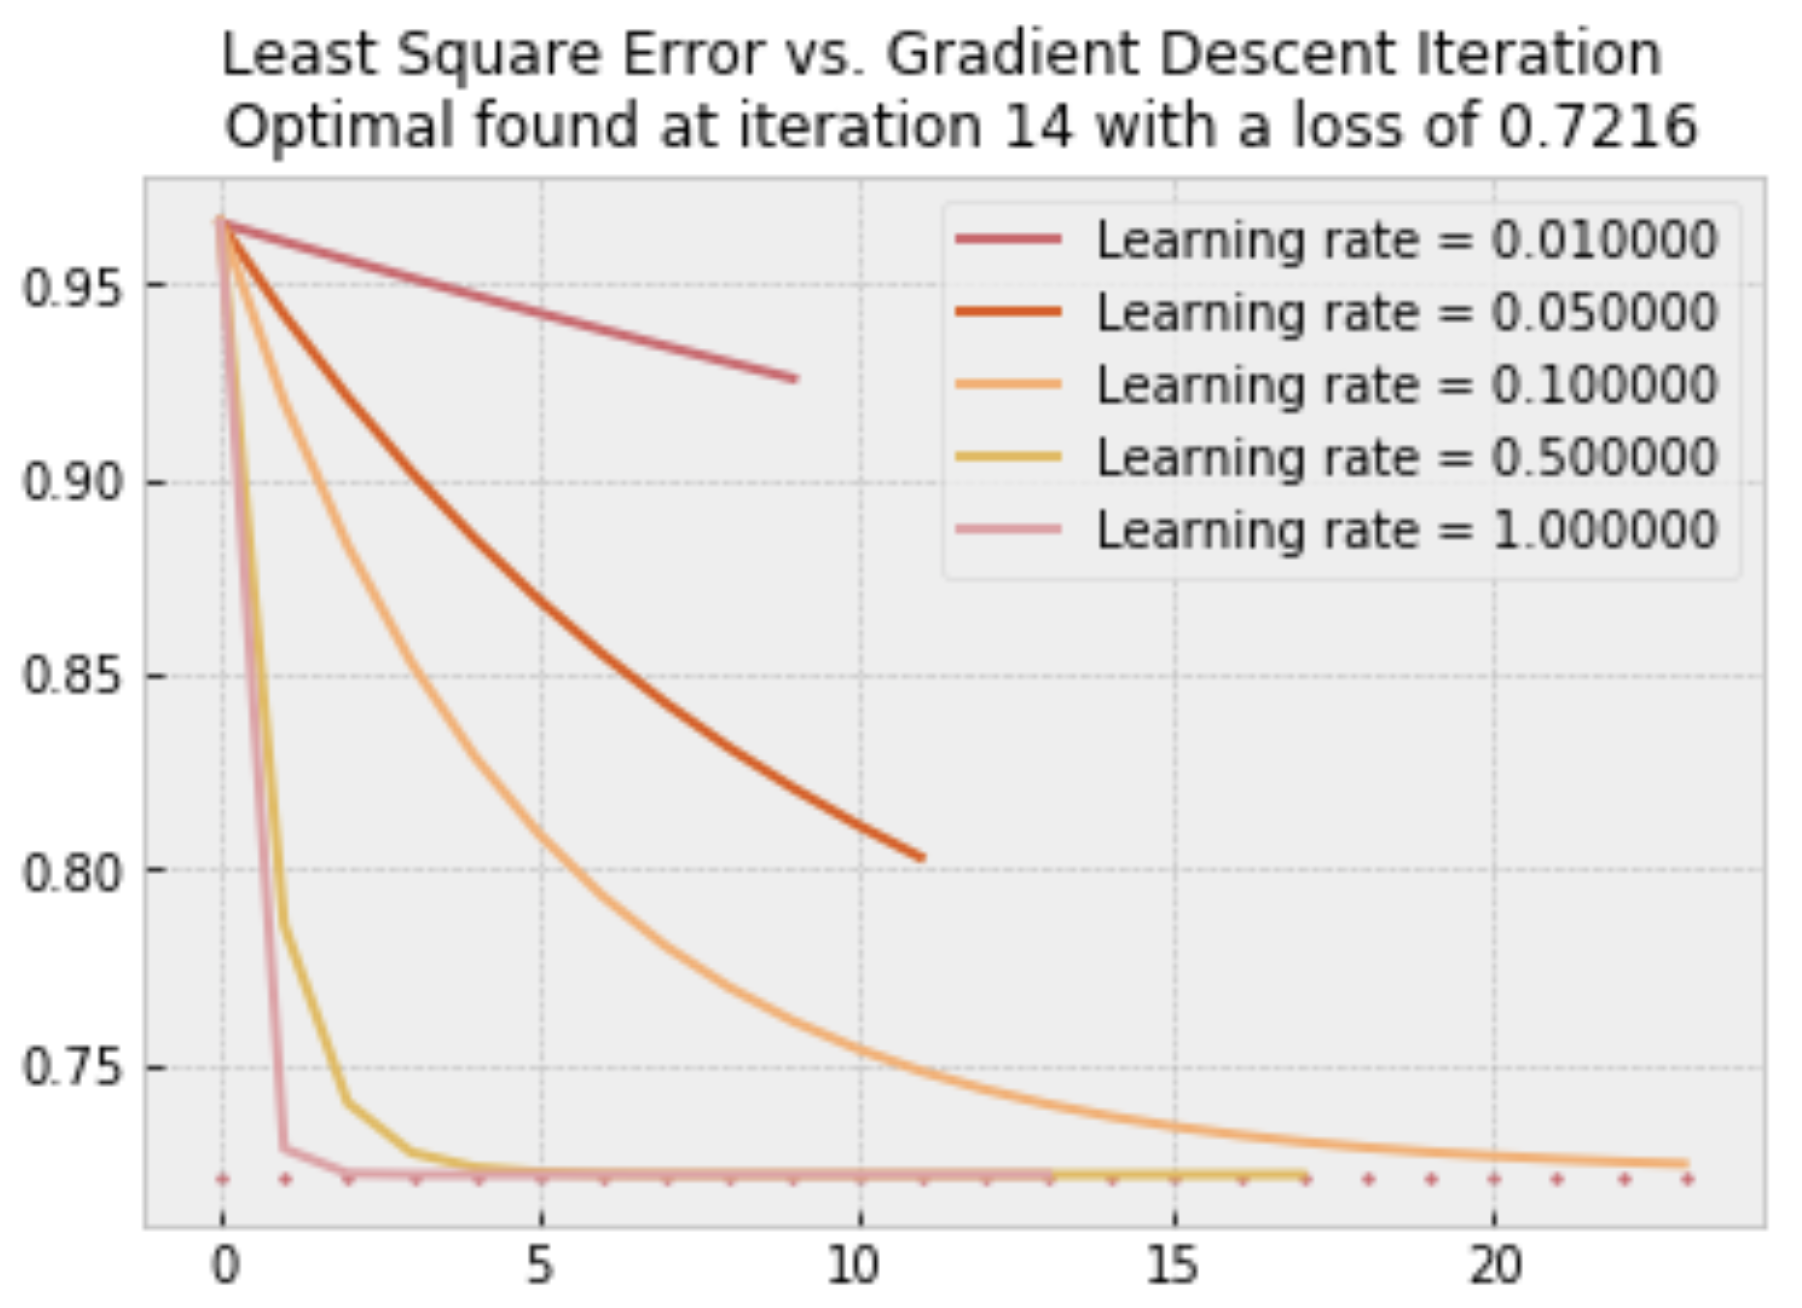
\includegraphics[width=\linewidth]{A3_1_1.png}
      \caption{Gradient Descent}
    \end{subfigure}
    \begin{subfigure}[b]{0.45\linewidth}
      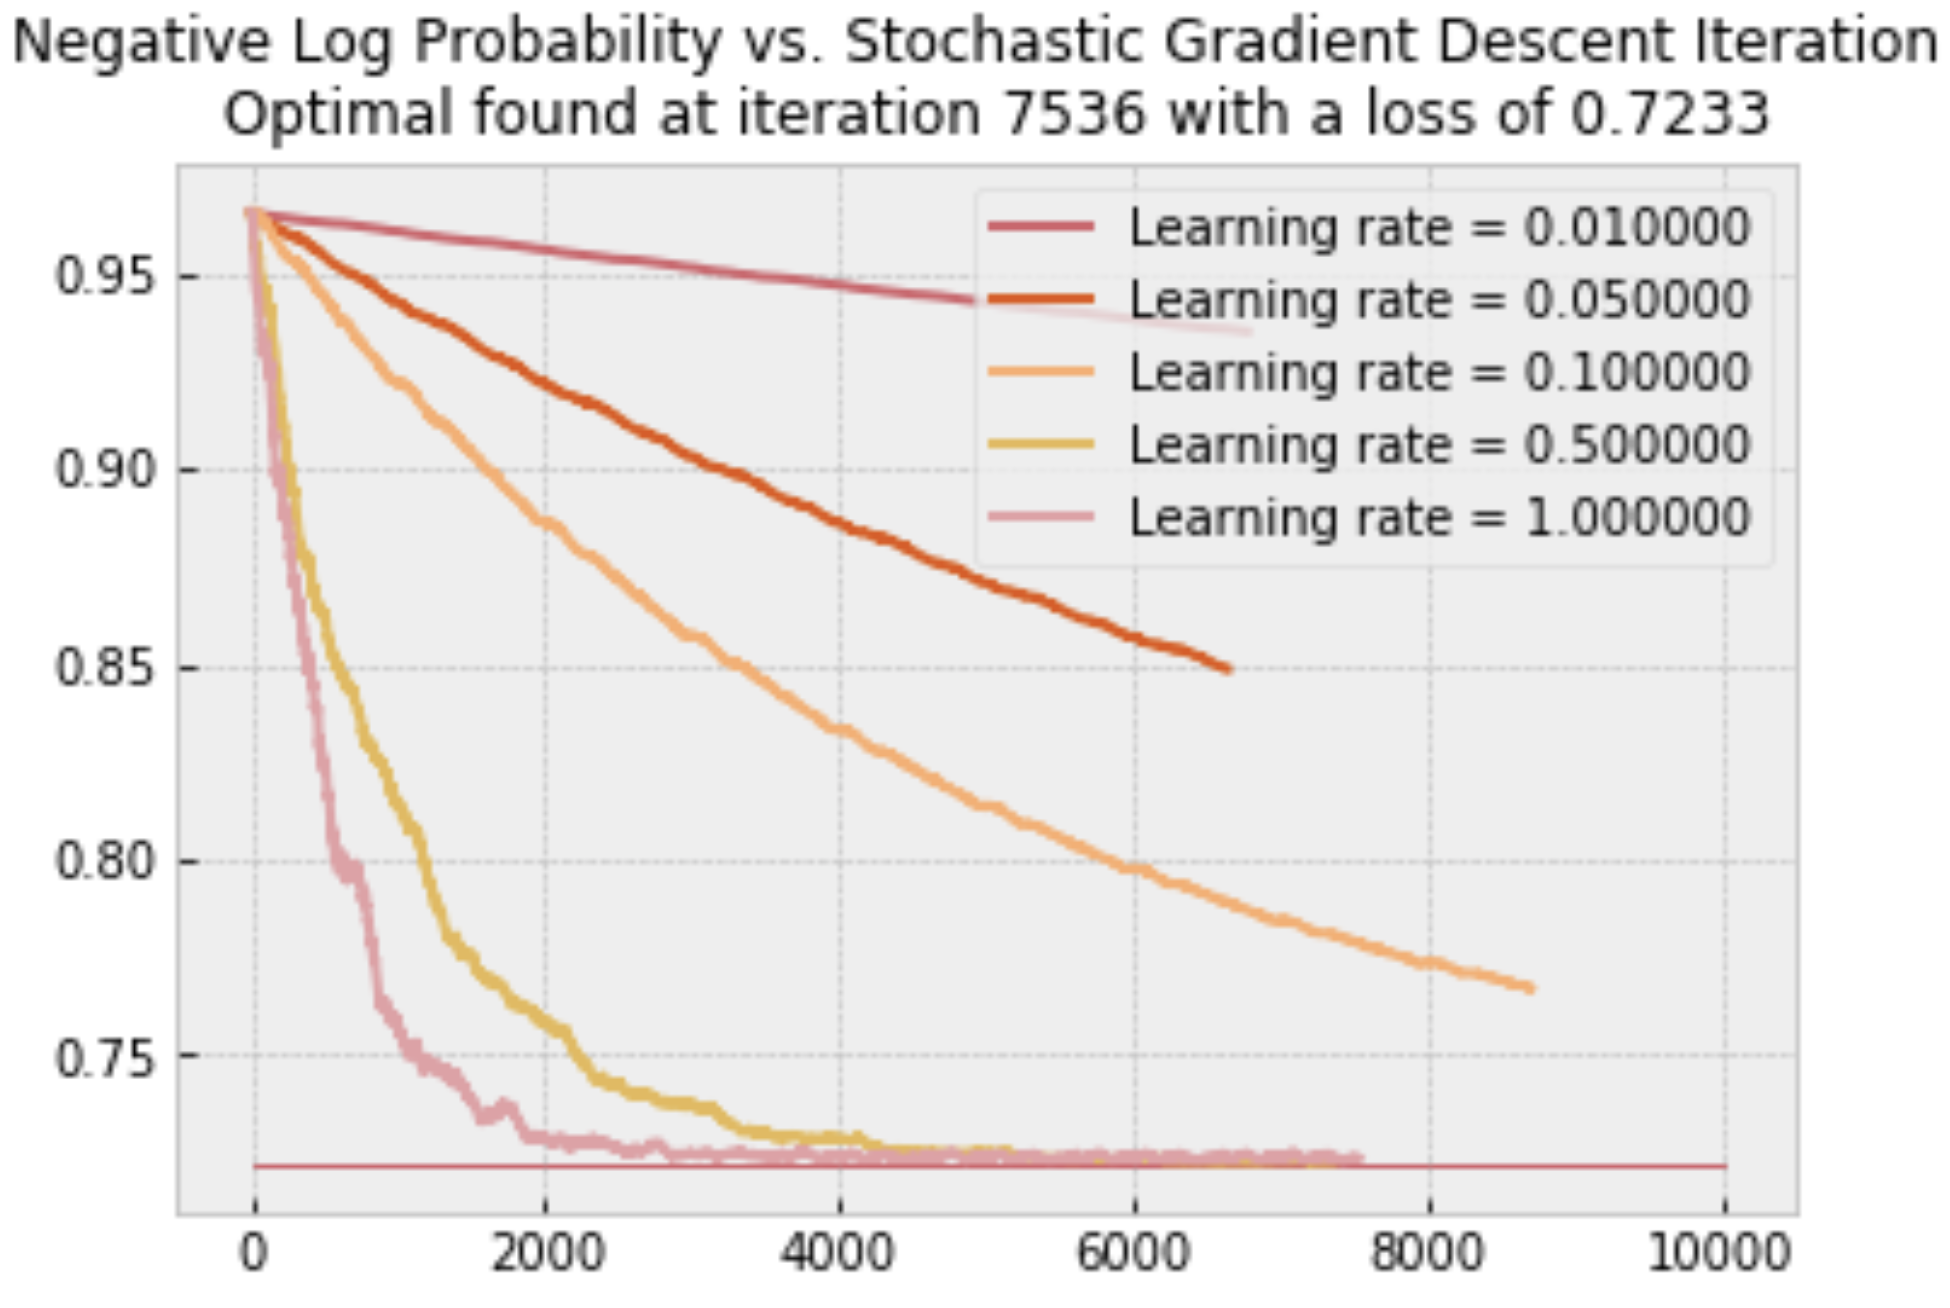
\includegraphics[width=\linewidth]{A3_1_2.png}
      \caption{Stochastic Gradient Descent}
    \end{subfigure}
    \caption{Loss vs. iteration with a relative convergence criteria}
    \label{fig:Q1_1}
  \end{figure}

  Another convergence way is to compare the loss with the exact optimal loss determined by SVD, and break out when their difference is smaller than the errorbound for a few times. Though in reality, calculating the SVD takes much more time and it completely misaligns with the purpose of Gradient Descent, this convergence criteria allows easier visualization of how long it takes for each algorithm/parameter to reach the minimum. Therefore, the following figures and performance outcome are all based on this convergence criteria.
  \begin{figure}[!h]
    \centering
    \begin{subfigure}[b]{0.45\linewidth}
      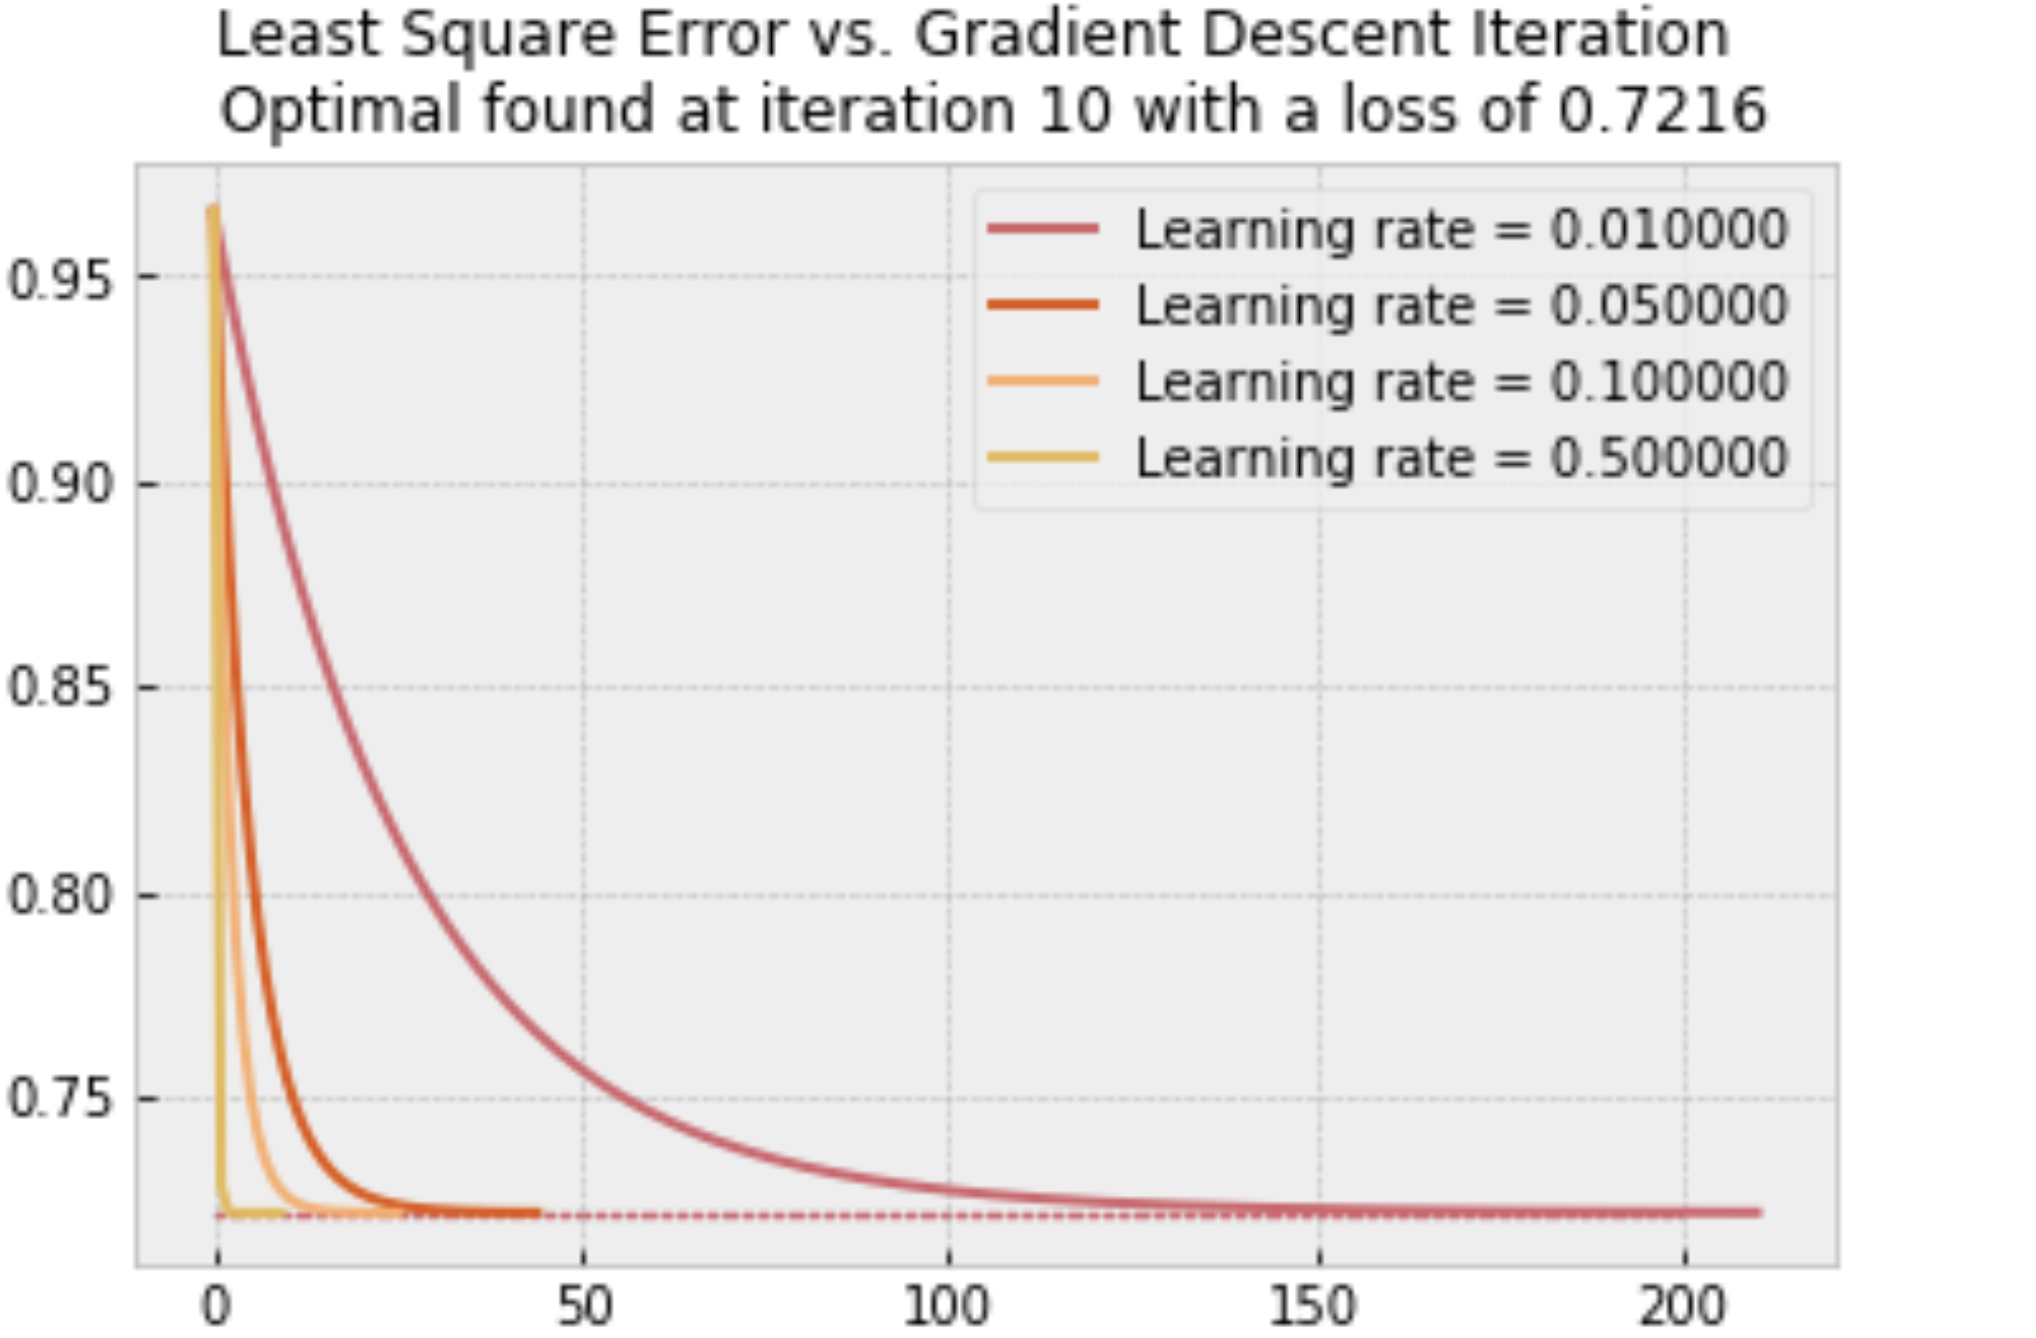
\includegraphics[width=\linewidth]{A3_1_3.png}
      \caption{Gradient Descent}
    \end{subfigure}
    \begin{subfigure}[b]{0.45\linewidth}
      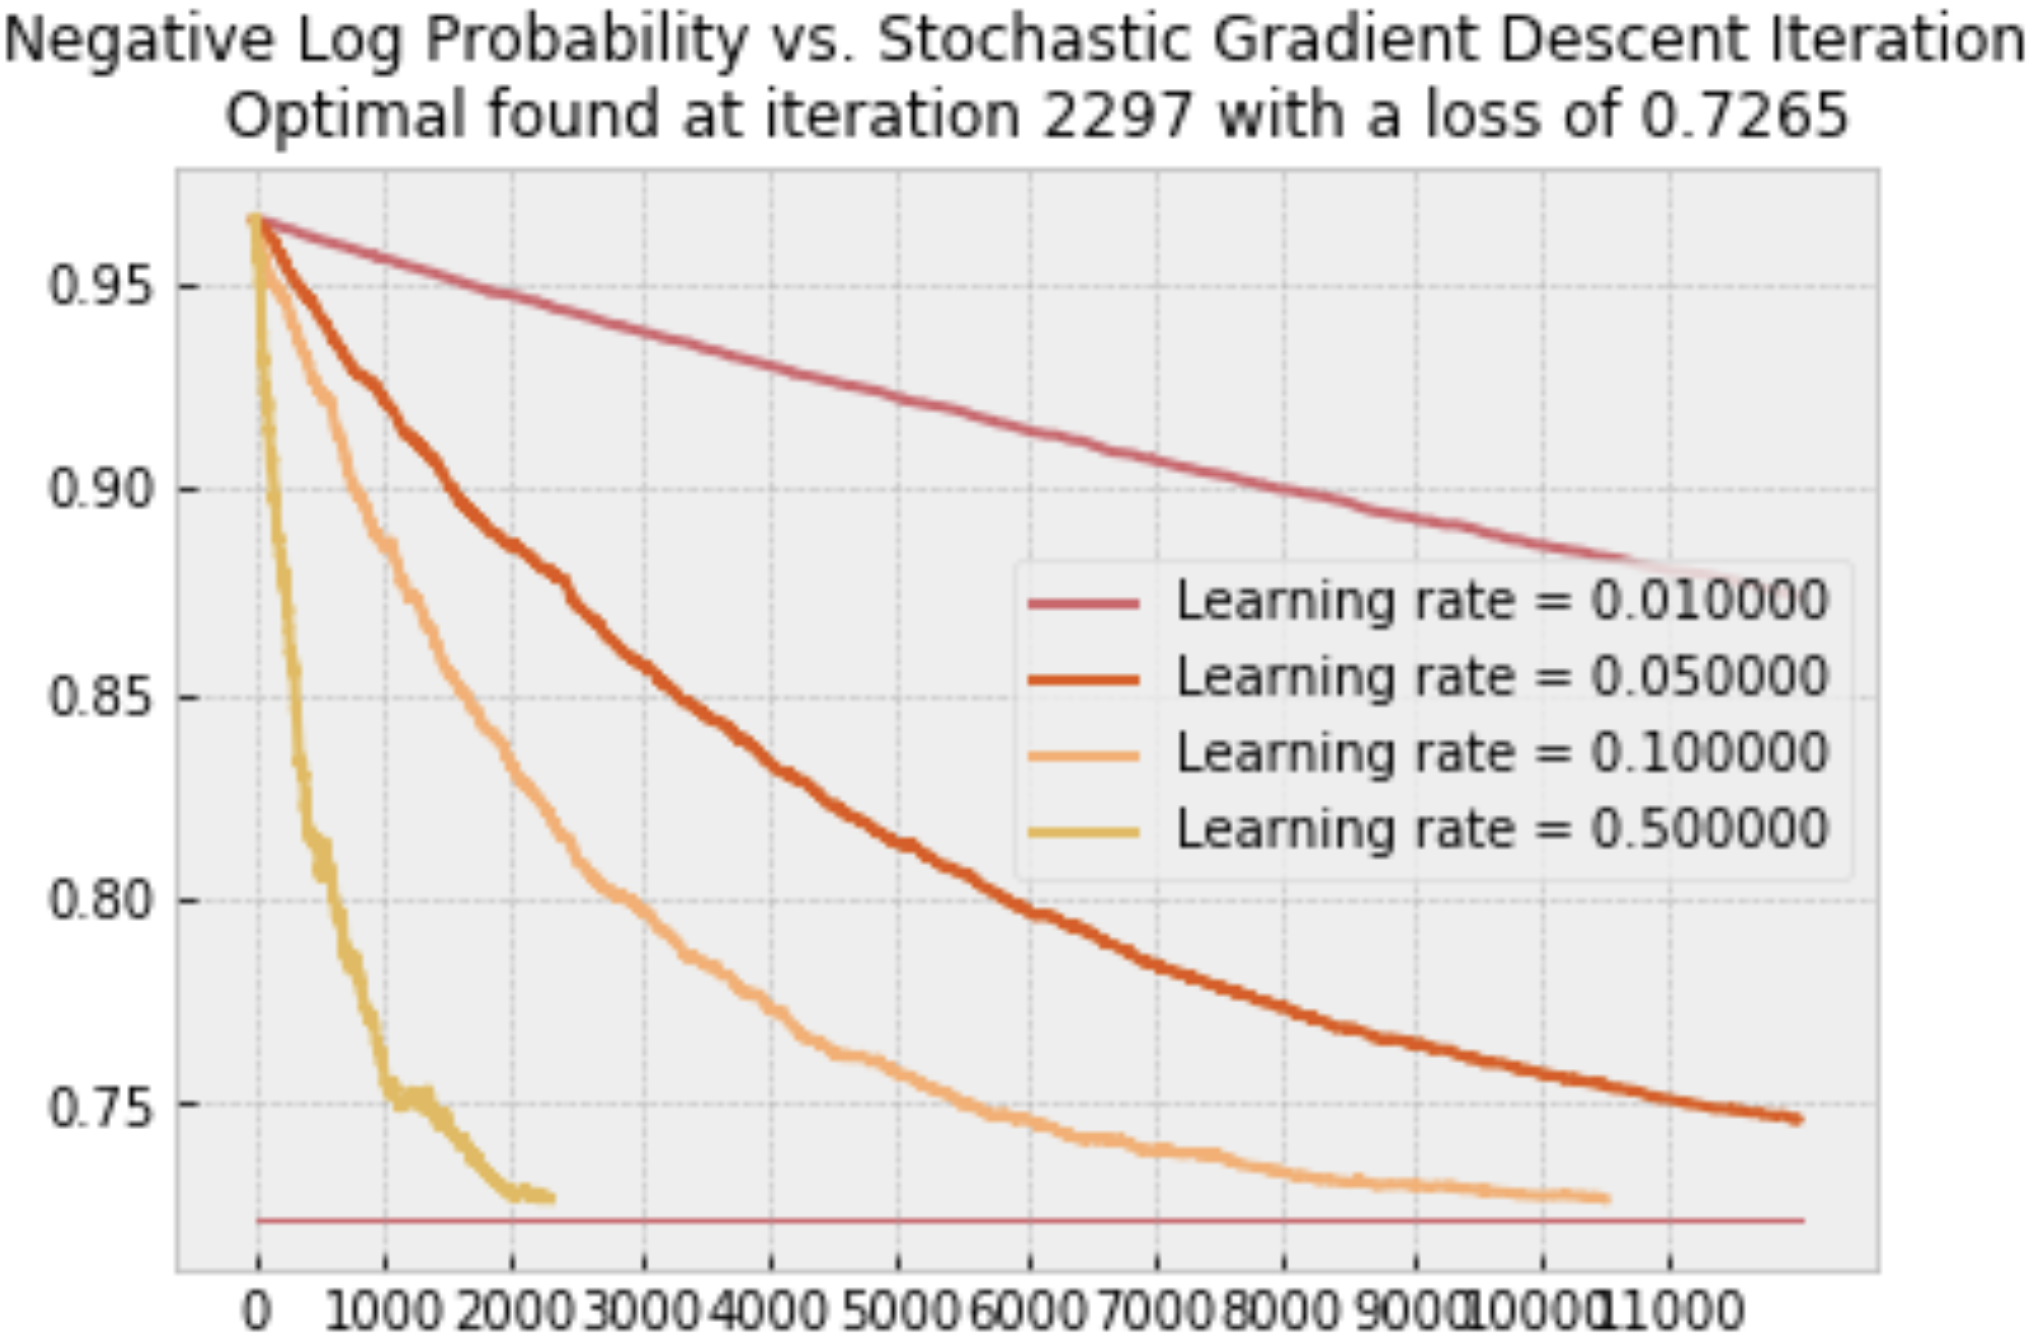
\includegraphics[width=\linewidth]{A3_1_4.png}
      \caption{Stochastic Gradient Descent}
    \end{subfigure}
    \caption{Loss vs. iteration with a absolute convergence criteria}
    \label{fig:Q1_2}
  \end{figure}

\vspace{0.2cm}
\textbf{Performance \& Optimal Learning Rate}

  The follwing table shows the number of iterations taken for the loss to be 0.005 away from the exact optimum loss of 0.722, 5 times for GD and 10 times for SGD. Note that the iterations in the table are "full-batch" ones while those shown in the figures are "mini-batch" ones for easier visualization, and only 12000 mini-batch (i.e. 12 full-batch) iterations are plotted for SVD so that the difference between different learing rates can be visualized more clearly.

  From the table, it is easy to see how mush faster it is for SGD to converge, compared to GD. When learning rate is 0.5, it converges to the exact optimal in about 2000 mini-batch iterations! In this case, 0.5 is the best learning rate if fastest convergence is the objective, since it converges the fastest without producing any huge up-and-downs. In addition, 0.01 is the best learning rate if minimum RMSE is the objective, but as the RMSEs differ by only 1-2\%, the fastest convergence makes a better objective.

  \begin{table}[!h]
  \centering
  \scalebox{0.74}{\begin{tabular}[t]{||r | c c | c c||}
    \hline
    \rowcolor{lightgray}\multicolumn{5}{||c||}{Convergence on "pumadyn32nm"}\\
            &  Gradient Descent & & Stochastic Gradient Descent & \\
    \hline
    Learning rate & Iterations & RMSE  &  Iterations & RMSE\\
    \hline
    0.01  & 211   & 0.8696 & 103.783      & 0.8667\\
    0.05  & 45    & 0.8699 & 20.637       & 0.8669\\
    0.1   & 26    & 0.8703 & 10.504       & 0.8672\\
    0.5   & 10    & 0.8706 & 2.297        & 0.8664\\
    \hline
  \end{tabular}}
  \caption{Iteration and RMSE performance with different learning rates}
  \end{table}


%----------------------------------------------------------------------------------------
%	PROBLEM 2
%----------------------------------------------------------------------------------------
\vspace{0.3cm}
\section*{Logistic Regression on Classification of Dataset Iris} % The * makes it an unnumbered section

\textbf{Convergence Criteria and Loss Function}

  The convergence criteria for logistic regression is the same as the one above, for better comparison and visualization between GD, SGD, and different parameters, shown in the Figure 3. The follwing table then shows the number of iterations taken for the loss to be 0.005 away from the exact optimum loss of 0.487, 5 times for GD and 10 times for SGD. Note that the loss function, as shown in the earlier part of report.

  In regards to the question about whether it is reasonable for the value of the log-likelihood if $\hat f(x^{(i)}; w) = 1$ but the correct label is $y^{(i)} = 0$ for some $i$, I think it is \textbf{not reasonble}. It can be counterproved by plugging the $\hat f$ and $y$ values into the log likelihood equation:
  $$log Pr(y|w, X) = \sum_{i=1}^{N-M}(y^{(i)}log(\hat f^{(i)}) + (1 - y^{(i)})log(1 - \hat f^{(i)})) + M(0 \cdot log(1) + 1 \cdot log(0))$$
  where M of the N data points have have the aforementioned properties,
  $$Pr(y|w, X) = 10^{Mlog(0) + \sum_{i=1}^{N-M}(y^{(i)}log(\hat f^{(i)}) + (1 - y^{(i)})log(1 - \hat f^{(i)}))} $$
  $$= 0^M \cdot 10^{\sum{i=1}^{N-M}(y^{(i)}log(\hat f^{(i)}) + (1 - y^{(i)})log(1 - \hat f^{(i)}))} = 0$$
  Inituitively, the total likelihood is the product of the $N$ likelihoods from all datapoints, so one being 0 means all being 0, as mathematically shown in the previous computation. However, it doesn't make sense if the likelihood of a set of prediction is completely impossible.

  To have a better sense of the order of magnitude of the errors, I nomalized the log likelihood by dividing the size of training points $N$ just like in the linear regression part, so the loss function in my algorithm is:
  $$L(w) = -\frac{1}{N}\sum{i=1}^N(y^{(i)}log(\hat f^{(i)}) + (1 - y^{(i)})log(1 - \hat f^{(i)}))$$

  Note that to align with the assignment, where the loss function isn't normalized, the actual stepsizes are $N$ times smaller than the ones shown in the figures, and the losses are also $N$ times larger. Though such scaling doesn't effect the shapes of the descent and performance, the numbers in the table below are scales by $N=104$ in accordance to the assignment.


\vspace{0.2cm}
\textbf{Performance \& Optimal Learning Rate}
  \begin{figure}[!h]
    \centering
    \begin{subfigure}[b]{0.45\linewidth}
      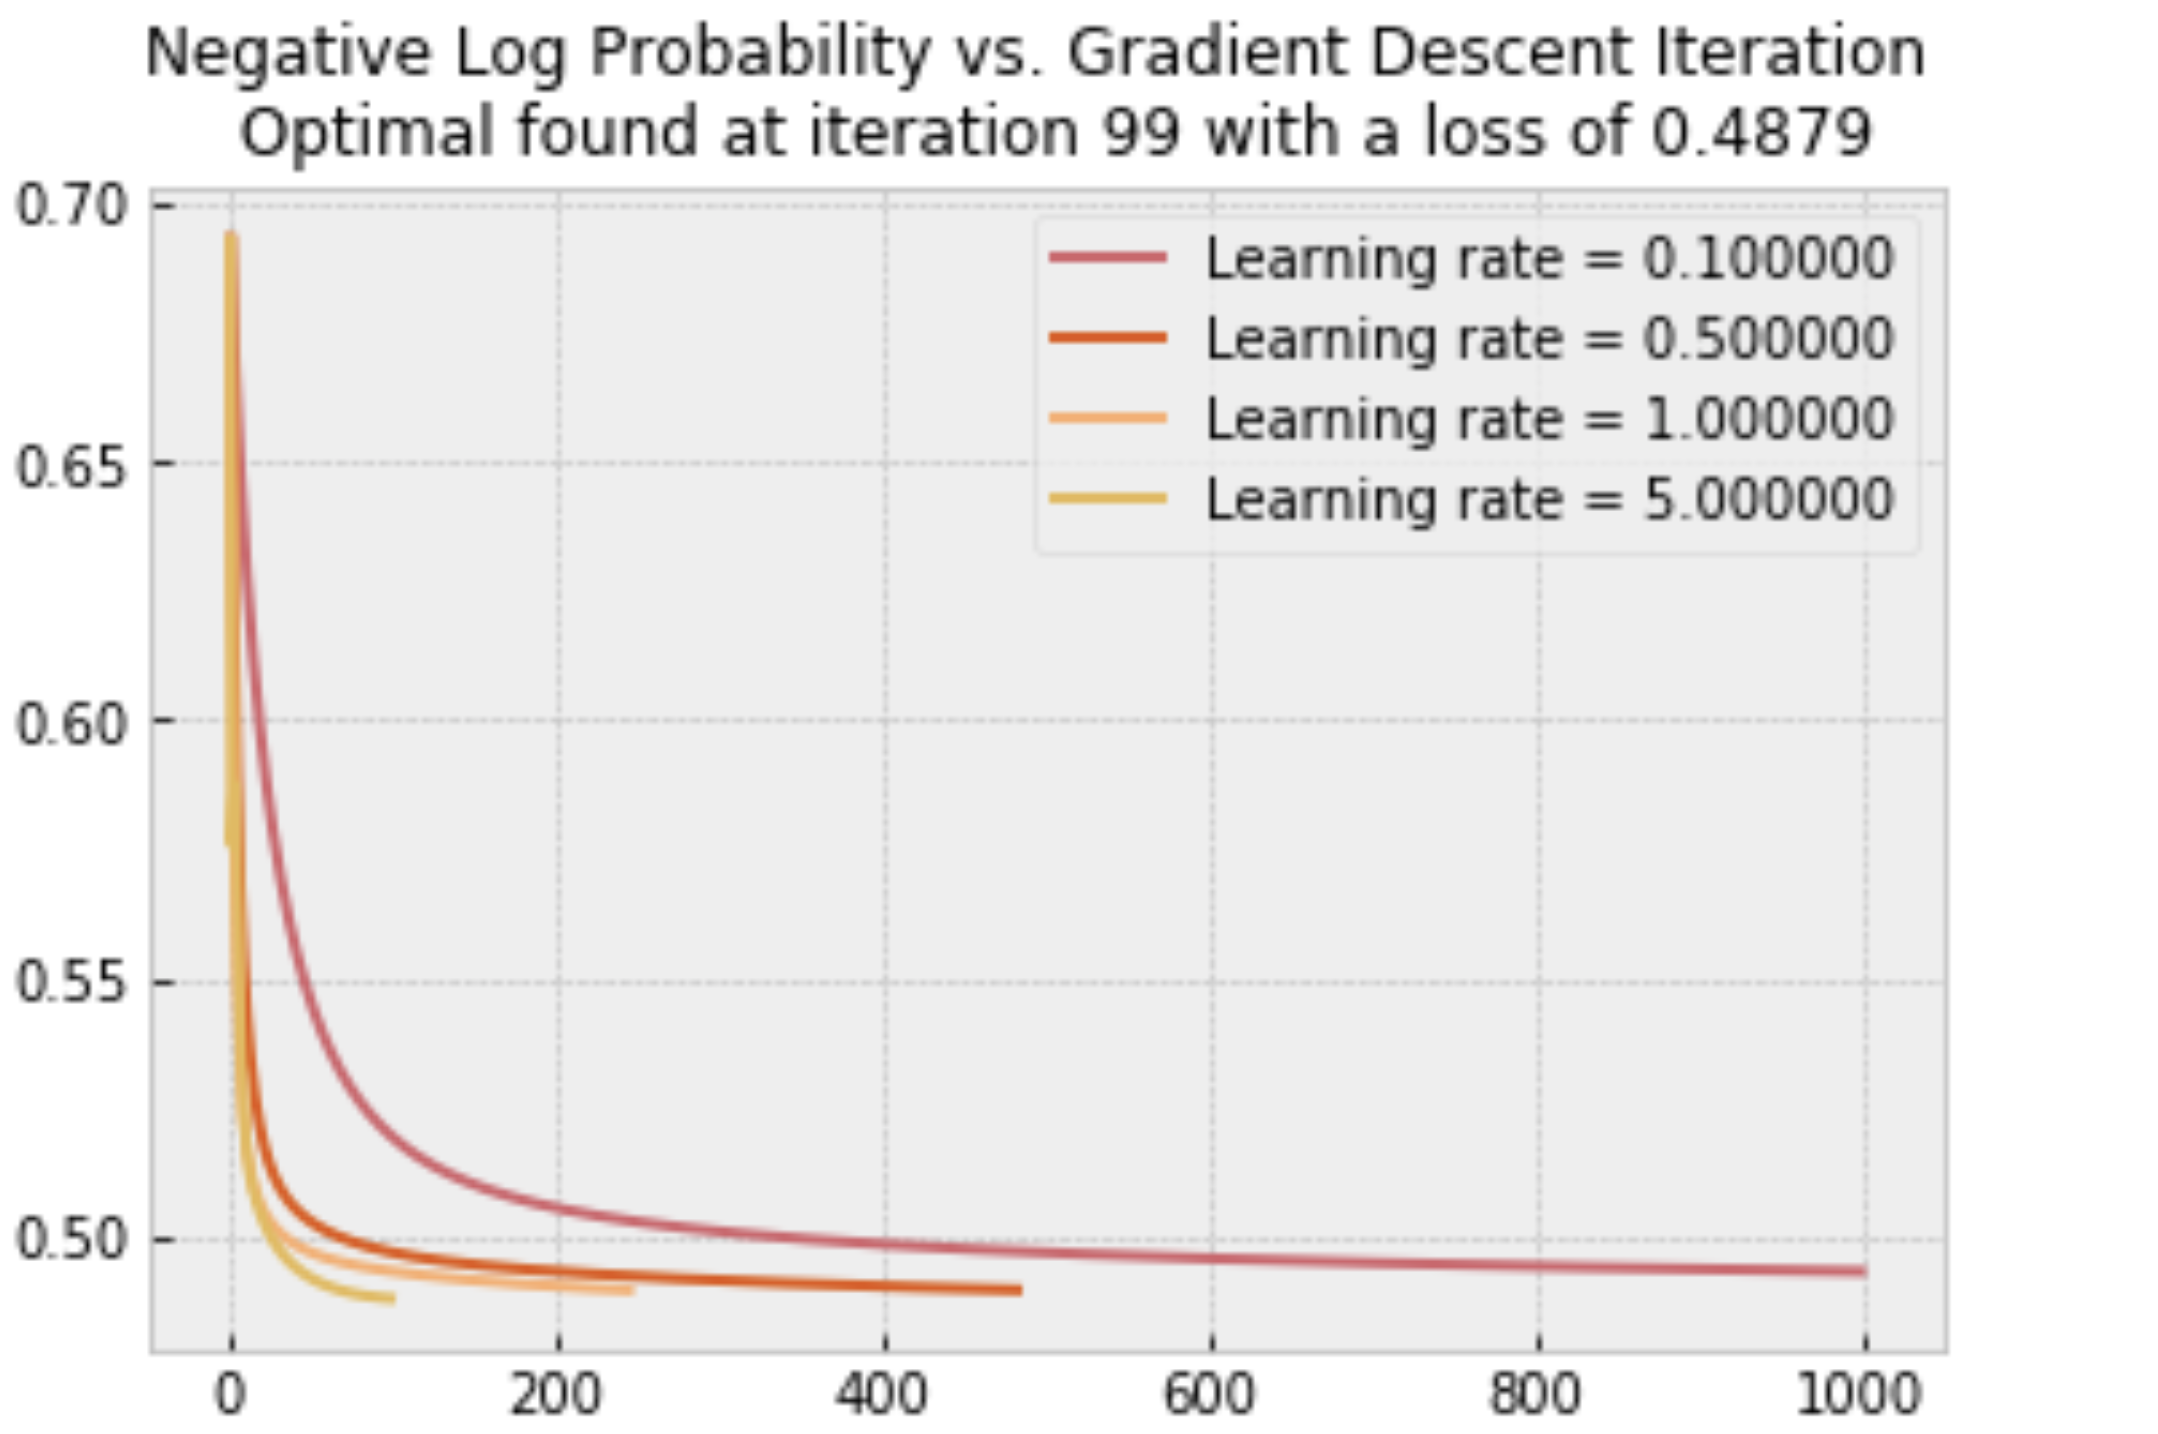
\includegraphics[width=\linewidth]{A3_2_1.png}
      \caption{Gradient Descent}
    \end{subfigure}
    \begin{subfigure}[b]{0.45\linewidth}
      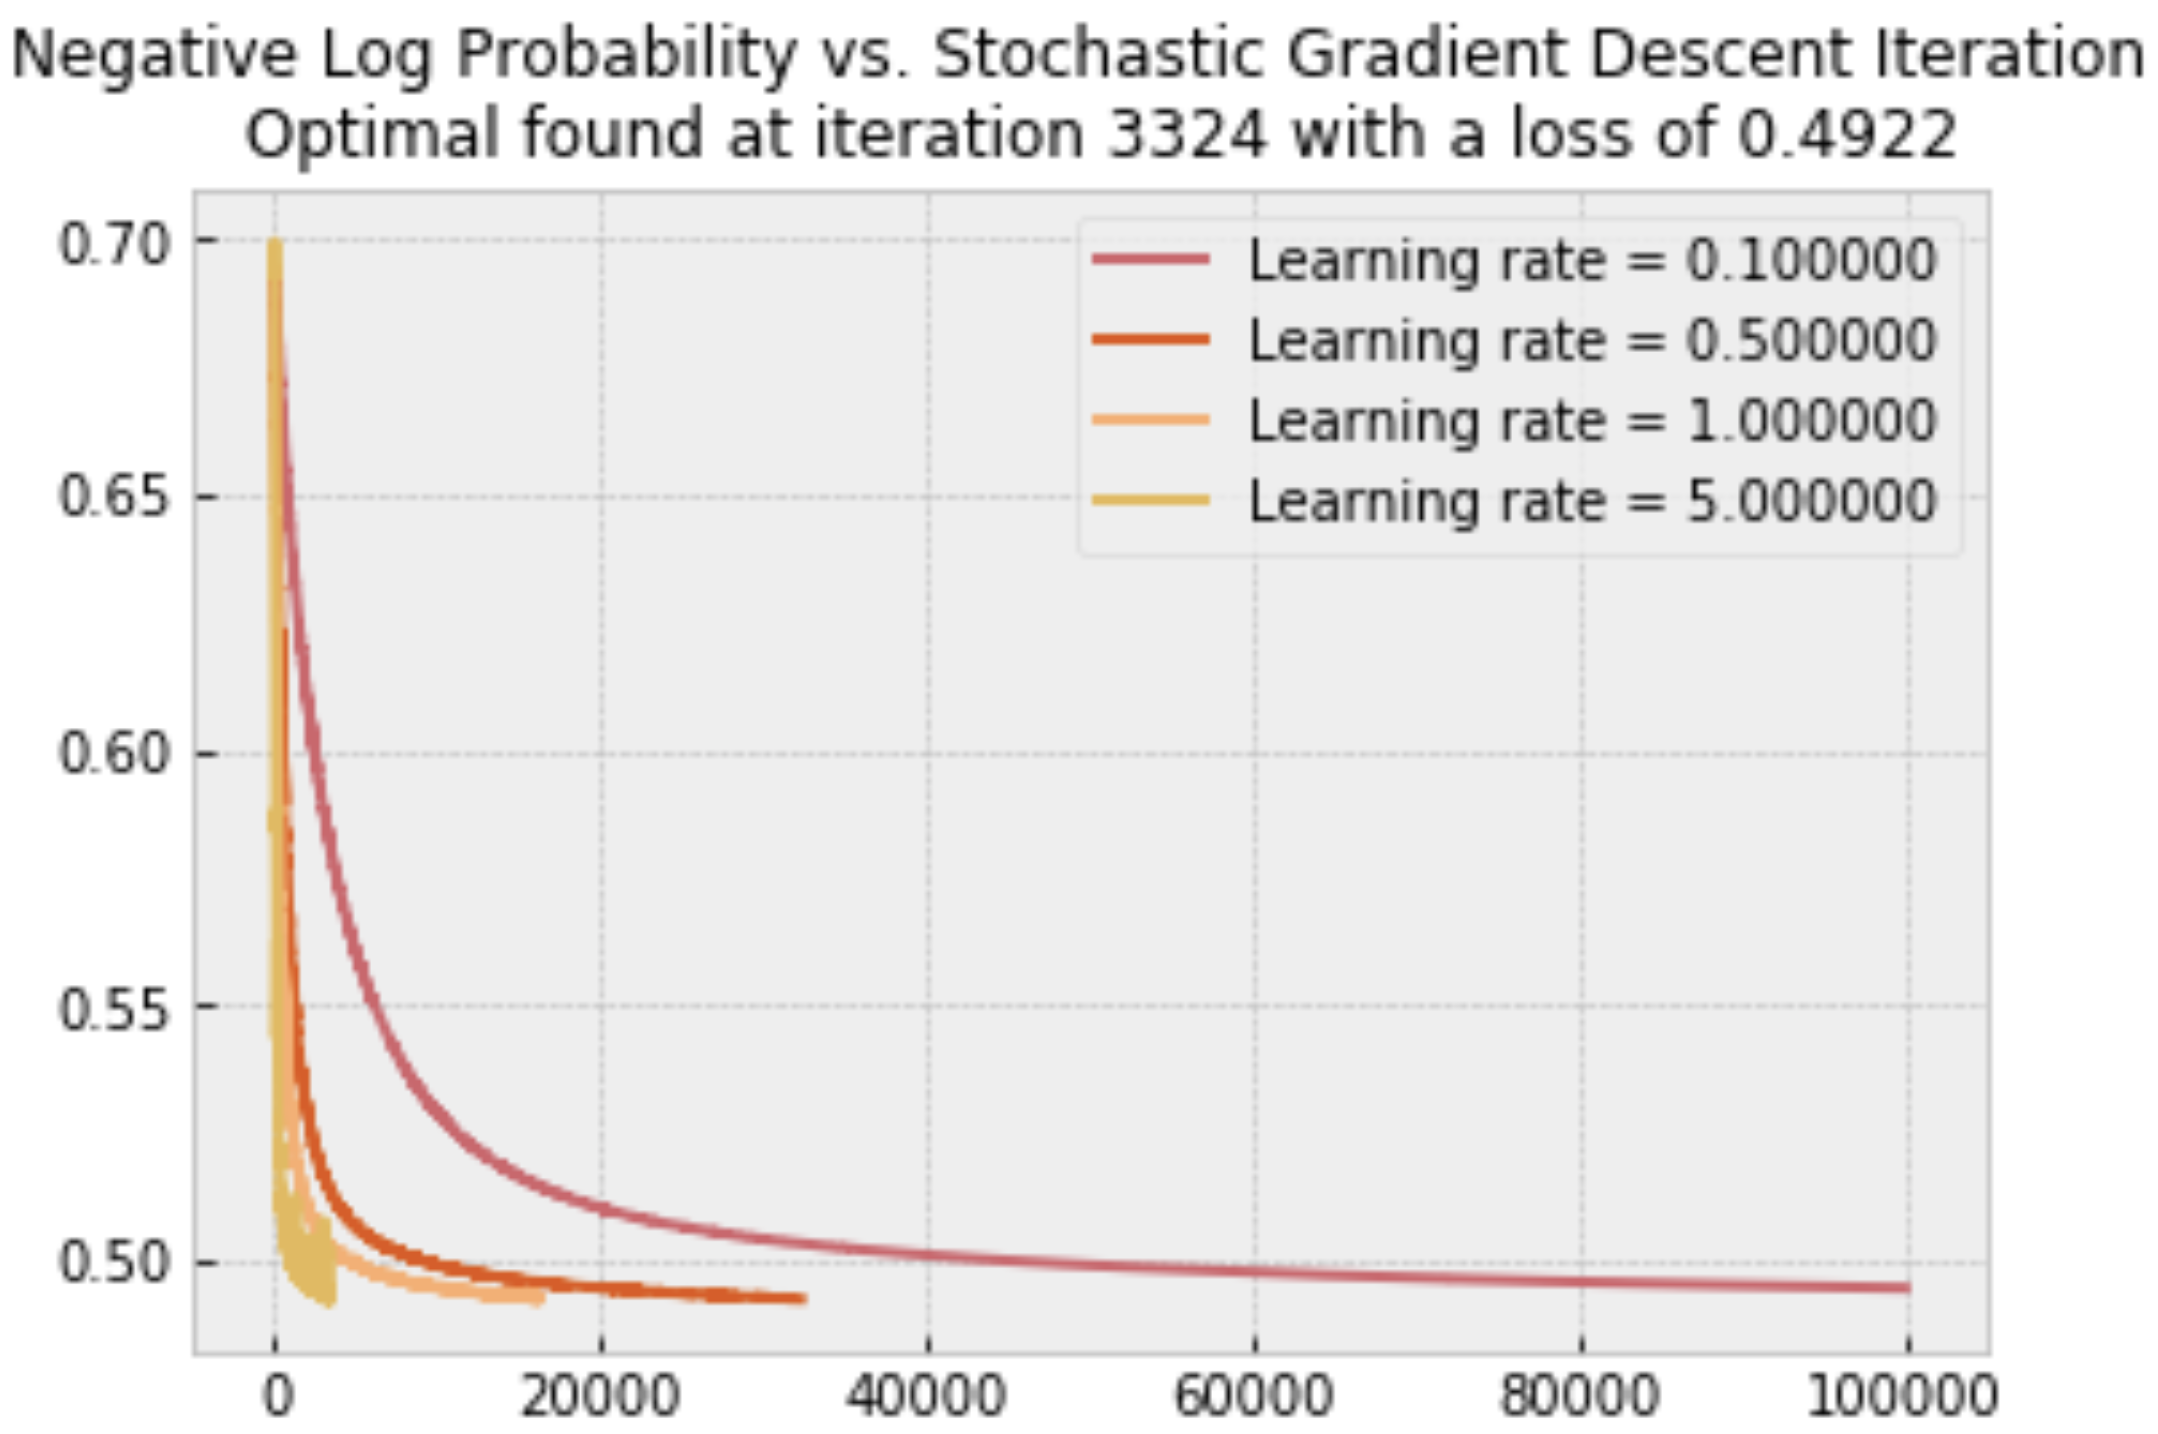
\includegraphics[width=\linewidth]{A3_2_2.png}
      \caption{Stochastic Gradient Descent}
    \end{subfigure}
    \caption{Negative log likelihood vs. iteration with a absolute convergence criteria}
    \label{fig:Q1_2}
  \end{figure}

  \begin{table}[!h]
  \centering
  \scalebox{0.74}{\begin{tabular}[t]{||r | c c c | c c c ||}
    \hline
    \rowcolor{lightgray}\multicolumn{7}{||c||}{Convergence on "Iris"}\\
            & & Gradient Descent & & & Stochastic Gradient Descent &  \\
    \hline
    Learning rate & Iterations & Log likelihood & Accuracy & Iterations & Log likelihood & Accuracy\\
    \hline
    0.001  & 1000   & -7.1390 &  73.3\% & 961.87   & -7.1218&  73.3\%   \\
    0.005  & 483    & -7.0719 &  66.7\% & 310.21   & -7.1287&  73.3\%   \\
    0.01   & 245    & -7.0699 &  66.7\% & 155.80   & -7.1260&  73.3\%   \\
    0.05   & 99     & -7.0481 &  66.7\% & 31.961   & -7.1111&  66.7\%   \\
  \hline
  \end{tabular}}
  \caption{Iteration and performance with different learning rates, with the un-normalized loss function}
  \end{table}

  The difference in the number of full-batch iterations taken to converge isn't as much as in the linear regression part, however, it is still obvious that SGD takes a fewer number of full-batch iterations to produce results that are even better than that of GD. In this case, the slowest learning rate of 0.001 generates the best accuracy but lowest likelihood, compared to the fastest 0.05 learning rate that generates the least accuracy but highest likelihood. In such a classification case, log likelihood is a better performance metric because:
  \begin{enumerate}
    \item For smaller test sets, the accuracy is very sensitive to the prediction of every point, as any True/False brings an extra point at one polar of the spectrum. As the log likelihood allows numbers in between, the impact of an outlier is significantly reduced.
    \item Because the classification is made by if the sigmoid function outputs a likelihood smaller or larger than 0.5. Therefore, using the log likelihood captures the values around 0.5 and reduces the penalty even if they give the wrong prediction, while accuracy ignores the fact that some predictions are only "almost" right/wrong and treats them all as "absolutely" right/wrong.
  \end{enumerate}
  With that being said, as the 0.05 dataset produces both a higher log likelihood and converges faster, it is considered the optimal learning rate amoung the four, for dataset Iris.


%----------------------------------------------------------------------------------------
%	PROBLEM 3
%----------------------------------------------------------------------------------------
% \vspace{0.3cm}
% \section*{Conclusion} % The * makes it an unnumbered section
% The k-nearest neighbors algorithm (k-NN) is experienced with different datasets to study its properties, whose results are summarized and discussed in this report. First, a 5-fold cross validation is performed on each dataset to choose the optimal k-NN parameters. The test results are generally consistant with the validation results for all the datasets other than "mauna\_loa", which is more suitable for linear regression due to its underlying data trend that cannot be recognized by k-NN.
%
% Broadcasting and k-d tree are then used to modify the k-NN implementation and they are testes "rosenbrock" with fixed k-NN parameters but various feature dimensions. It is observed that k-d tree is the fastest with low dimension datasets and half vectorization of the testing points performs the best for higher dimensions. Either way, any extent of vectorization is shown to be faster than the brutal force k-NN with two loops.
%
% In comparison to linear regression, k-NN performs significantly better in classification, though with a much slower speed. In terms of regression, k-NN's accuracy varies with different datasets, as it depends on the distribution of data points: a randomly/uniformly distributed dataset allows k-NN to make good predictions while a trendy one is better with linear regression, and the worst is a test set whose features are out of the boundary of the training points, such as "mauna\_loa".
\end{document}
